\documentclass[12pt]{scrartcl}

\usepackage{blindtext}
\usepackage{multicol}
\usepackage[a4paper, total={19cm, 27cm}]{geometry}
\usepackage{times}
\renewcommand{\familydefault}{\sfdefault}
\usepackage{graphicx}
\usepackage{parskip}
\usepackage{amsmath}
\usepackage{steinmetz}

\graphicspath{ {./PrintsQuestoes/} }

\pagenumbering{gobble}

\begin{document}

% \begin{multicols}{2}

    \section*{Problema P9.77}

    \begin{center}
        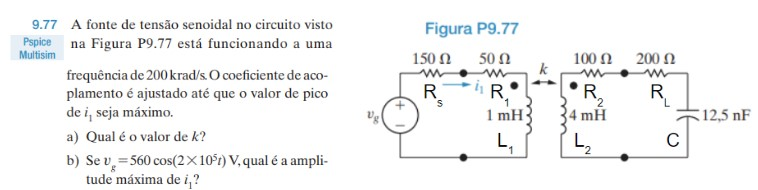
\includegraphics[scale=1.0]{P9.77.jpg}
    \end{center}

    \subsection*{(a)}

    O valor de \(i(t)\) depende da impedância \(Z_{in}\) vista pela fonte \(V_{g}\).
    Sabemos que \(Z_{in}\) é expressa por

    \begin{equation}\label{eq:1}
        Z_{in} = Z_{11} + Z_{r}
    \end{equation}

    Além disso, sabemos que a impedância refletida \(Z_{r}\) é dada por

    \begin{equation}\label{eq:2}
        Z_{r} = \frac{\omega^2M^2}{Z_{22}}
    \end{equation}

    Substituindo (\ref{eq:2}) em (\ref{eq:1}), temos

    \begin{equation}\label{eq:3}
        Z_{in} = Z_{11} + \frac{\omega^2M^2}{Z_{22}}
    \end{equation}

    Onde
    \begin{itemize}
        \item \(Z_{11}\): Autoimpedância da malha do primeiro enrolamento;
        \item \(Z_{22}\): Autoimpedância da malha do segundo enrolamento;
        \item \(M\): Indutância mútua.
    \end{itemize}

    Expandindo os termos de (\ref{eq:3}), temos

    \begin{equation}\label{eq:4}
        Z_{in} = R_s + R_1 + j \omega L_1 + \frac{\omega^2(k\sqrt{L_1L_2})^2}{j\omega L_2 + R_2 + R_L + \frac{1}{j\omega C}}
    \end{equation}

    Vamos reescrever (\ref{eq:4}) de modo a isolar a parte real da parte complexa.

    \[ Z_{in} = R_s + R_1 + j \omega L_1 + \frac{\omega^2k^2L_1L_2}{j\omega L_2 + R_2 + R_L - \frac{j}{\omega C}} \]

    \[ Z_{in} = R_s + R_1 + j \omega L_1 + \frac{\omega^2k^2L_1L_2}{R_2 + R_L + j(\omega L_2 - \frac{1}{\omega C})} \]

    \[ Z_{in} = R_s + R_1 + j \omega L_1 + \frac{(\omega^2k^2L_1L_2)(R_2 + R_L - j(\omega L_2 - \frac{1}{\omega C}))}{(R_2 + R_L + j(\omega L_2 - \frac{1}{\omega C}))(R_2 + R_L - j(\omega L_2 - \frac{1}{\omega C}))} \]

    \[ Z_{in} = R_s + R_1 + j \omega L_1 + \frac{(\omega^2k^2L_1L_2)(R_2 + R_L) - j(\omega^2k^2L_1L_2)(\omega L_2 - \frac{1}{\omega C})}{(R_2 + R_L)^2 + (\omega L_2 - \frac{1}{\omega C})^2} \]

    \begin{equation}\label{eq:5}
        Z_{in} = R_s + R_1 + \frac{(\omega^2k^2L_1L_2)(R_2 + R_L)}{(R_2 + R_L)^2 + (\omega L_2 - \frac{1}{\omega C})^2} + j \left(\omega L_1 - \frac{(\omega^2k^2L_1L_2)(\omega L_2 - \frac{1}{\omega C})}{(R_2 + R_L)^2 + (\omega L_2 - \frac{1}{\omega C})^2}\right)
    \end{equation}

    A partir de (\ref{eq:5}) podemos determinar o módulo de \(Z_{in}\).

    \begin{equation}\label{eq:6}
        |Z_{in}|(k) = \sqrt{\left(R_s + R_1 + \frac{(\omega^2k^2L_1L_2)(R_2 + R_L)}{(R_2 + R_L)^2 + (\omega L_2 - \frac{1}{\omega C})^2}\right)^2 + \left(\omega L_1 - \frac{(\omega^2k^2L_1L_2)(\omega L_2 - \frac{1}{\omega C})}{(R_2 + R_L)^2 + (\omega L_2 - \frac{1}{\omega C})^2}\right)^2}
    \end{equation}

    A expressão (\ref{eq:6}) expressa o módulo de \(Z_{in}\) como uma função do coeficiente \(k\). O valor máximo de \(i(t)\) ocorre quando \(Z_{in}(k)\) aitinge seu valor mínimo, ou seja, quando

    \begin{equation}\label{eq:7}
        \frac{d}{dk}|Z_{in}|(k) = 0
    \end{equation}

    Vamos diferenciar (\ref{eq:6}) com respeito a \(k\). Antes disso, vamos adotar uma notação para reduzir o tamanho da expressão.\newline
    Sejam

    \[ A = \frac{(\omega^2L_1L_2)(R_2 + R_L)}{(R_2 + R_L)^2 + (\omega L_2 - \frac{1}{\omega C})^2} \]

    e 

    \[ B = \frac{(\omega^2L_1L_2)(\omega L_2 - \frac{1}{\omega C})}{(R_2 + R_L)^2 + (\omega L_2 - \frac{1}{\omega C})^2} \]

    Note que  \(A\) e \(B\) não dependem de \(k\). Assim, podemos reescrever (\ref{eq:6}) como

    \begin{equation}\label{eq:8}
        |Z_{in}|(k) = \sqrt{\left(R_s + R_1 + A k^2\right)^2 + \left(\omega L_1 - B k^2\right)^2}
    \end{equation}

    Diferenciando (\ref{eq:8}) com respeito a \(k\), temos

    \begin{equation}\label{eq:9}
         \frac{d}{dk}|Z_{in}|(k) = \frac{1}{2}\frac{1}{\sqrt{\left(R_s + R_1 + A k^2\right)^2 + \left(\omega L_1 - B k^2\right)^2}} \left(2(R_s + R_1 + A k^2)(2Ak) + 2(\omega L_1 - B k^2)(2Bk)\right)
    \end{equation}

    Para que (\ref{eq:9}) seja igual a zero, temos

    \[ 2(R_s + R_1 + A k^2)(2Ak) + 2(\omega L_1 - B k^2)(-2Bk) = 0 \]

    \[ (R_s + R_1 + A k^2)(Ak) + (\omega L_1 - B k^2)(-Bk) = 0 \]

    \[ AkR_s + AkR_1 + A^2k^3 - \omega BkL_1 + B^2k^3 = 0 \]

    \[ k^3(A^2+B^2) + k(AR_s + AR_1 - \omega BL_1) = 0 \]

    \[ k\left(k^2(A^2+B^2) + (AR_s + AR_1 - \omega BL_1)\right) = 0 \]

    \[ k^2(A^2+B^2) + AR_s + AR_1 - \omega BL_1 = 0 \]

    \[ k = \sqrt{\frac{\omega BL_1 - AR_s - AR_1 }{(A^2+B^2)}} \]

    Substituindo os valores todos, temos

    \[ A = 192 \]

    \[ B = 256 \]

    \[ \boxed{k = 0.3536} \]

    \subsection*{(b)}

    Conhecido o valor de \(k = 0.3536\), podemos calcular o valor da impedância vista pela fonte através de (\ref{eq:4}), obtendo

    \[ Z_{in} = 224 + j168 \; \Omega \]

    Portanto, usando o fato que a corrente forncecida pela fonte é 

    \[ i(t) = \frac{v_g(t)}{Z_{in}} \]

    Em notação fasorial,

    \[ I = \frac{V_g}{Z_{in}} = \frac{\frac{560}{\sqrt{2}}\phase{0^{\circ}}}{224 + j168 \; \Omega} \]

    \[ I = 1.4142\phase{-36.57^{\circ}} \; A \]

    Portanto, o valor de pico de \(i(t)\) é

    \[ \boxed{i_m(t) = 1.4142 \sqrt{2} = 2 \; A}  \]


% \end{multicols}


\end{document}